\section{Optimointimenetelmät}

Konekoodiksi kääntäminen tuo ongelmaksi hitaan käännösvaiheen. Tämän takia modernit virtuaalikoneet sisältävät useamman kuin yhden kerroksen kääntäjiä eritasoisilla optimoinneilla. Tässä luvussa esitellään muutamia keinoja, joilla JavaScript-virtuaalikoneet ovat parantaneet kääntäjien suorituskykyä sekä niiden tuottaman konekoodin tehokkuutta.

\subsection{Piiloluokat}

\textit{Piiloluokat} (hidden classes)~\cite{v8design} ovat staattisia, eli muuttumattomia luokkia, joita virtuaalikone käyttää dynaamisten JavaScript-objektien kuvaamiseen. Jos objektia muutetaan, esimerkiksi lisäämällä siihen uusi \textit{ominaisuus} (property), luodaan sille uusi piiloluokka. Tämä kuulostaa järjettömältä kielen dynaamisuuden takia, mutta piiloluokkien hyödyt tulevat esiin, kun ohjelmassa on paljon samanlaisia objekteja, jotka pystyvät siten hyödyntämään samaa piiloluokkaa.

Kuvassa~\ref{fig:hiddenclass} näkyy esimerkki Piste-nimisen objektin ja sen piiloluokan muodostus. Kun konstruktorifunktiota kutsutaan, luodaan tyhjä objekti, jota virtuaalikone kuvaa piiloluokalla \textbf{C0}. Konstruktorissa objektiin liitetään ominaisuus x, jolloin virtuaalikone luo uuden piiloluokan \textbf{C1} ja lopulta y:n lisäyksen jälkeen \textbf{C2}:n. Seuraavalla kerralla kun luodaan uusi Piste-objekti, voidaan käyttää hyväksi olemassaolevia piiloluokkia.

\begin{figure}[ht]
    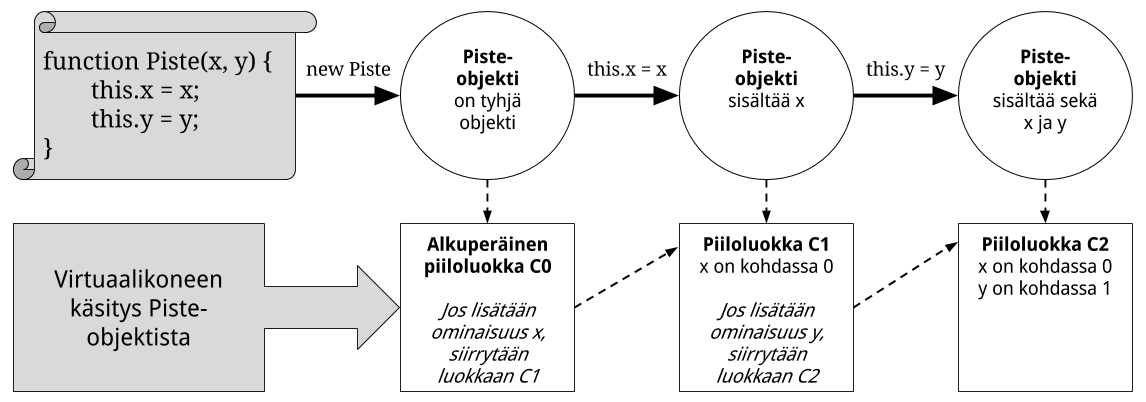
\includegraphics[width=\textwidth]{hidden-classes}
    \caption{Esimerkki piiloluokkien toimintaperiaatteesta}
     \centering
     \label{fig:hiddenclass}
\end{figure}

Piiloluokan ansiosta virtuaalikone tietää suoraan mistä muistipaikasta tieto löytyy hitaan \textit{hakurakenteen} (associative array) sijaan. Virtuaalikone voi generoida tehokkaampaa konekoodia, koska muistiviittaukset nopeutuvat huomattavasti.

\subsection{Välimuistit}

% Inline cache

\subsection{Roskienkeräys}

%(Garbage collection)

\subsection{Staattinen kertasijoitusmuoto}

%(Static single assignment form, SSA)